\documentclass[notes,10pt, aspectratio=169]{beamer}

\usepackage{pgfpages}
% These slides also contain speaker notes. You can print just the slides,
% just the notes, or both, depending on the setting below. Comment out the want
% you want.
% Note visibility is selected after package loading at the end of this preamble.
%\setbeameroption{show only notes} % Only notes
%\setbeameroption{show notes on second screen=right} % Both

\usepackage{helvet}
\usepackage[default]{lato}
\usepackage{array}
\usepackage{eurosym}
\usepackage{setspace}
\usepackage{animate}
\usepackage{multicol}
\usepackage{breqn}
\usepackage{subcaption}
\usepackage{caption}
\captionsetup{font=scriptsize, justification=raggedright,singlelinecheck=false}
\usepackage[export]{adjustbox}
\usepackage[scale=2]{ccicons}
\usepackage{tikz}
\newenvironment{wideitemize}{\itemize\addtolength{\itemsep}{10pt}}{\enditemize}
\usepackage{natbib}

\usepackage{tikz}
\usepackage{verbatim}
\setbeamertemplate{note page}{\pagecolor{yellow!5}\insertnote}
\usepackage{amsmath}
\usepackage{bm}
%\usepackage{mathpazo}
\usepackage{hyperref}
\usepackage{lipsum}
\usepackage{multimedia}
\usepackage{multirow}
\usepackage{graphicx}
\usepackage{dcolumn}
\usepackage{bbm}
\newcolumntype{d}[0]{D{.}{.}{5}}

\usepackage{changepage}
\usepackage{appendixnumberbeamer}
% \newcommand{\beginbackup}{
%   \newcounter{framenumbervorappendix}
%   \setcounter{framenumbervorappendix}{\value{framenumber}}
%   \setbeamertemplate{footline}
%   {
%      \leavevmode%
%      \hline
%      box{%
%       \begin{beamercolorbox}[wd=\paperwidth,ht=2.25ex,dp=1ex,right]{footlinecolor}%
% %         \insertframenumber  \hspace*{2ex}
%       \end{beamercolorbox}}%
%      \vskip0pt%
%   }
%  }

 \setbeamertemplate{footline}{
    \hbox{%
    \begin{beamercolorbox}[wd=\paperwidth,ht=3ex,dp=1.5ex,leftskip=2ex,rightskip=2ex]{page footer}%
        %\usebeamerfont{title in head/foot}%
        %\insertshorttitle \hfill
        %\insertsection \hfill
        %\tableofcontents[currentsection] \hfill
        \insertsectionnavigationhorizontal{0.7\paperwidth}{}{} \hfill
        \insertframenumber{} / \inserttotalframenumber
    \end{beamercolorbox}}%
}
\newcommand{\backupend}{
   \addtocounter{framenumbervorappendix}{-\value{framenumber}}
   \addtocounter{framenumber}{\value{framenumbervorappendix}}
}


\usepackage{graphicx}
\usepackage[space]{grffile}
\usepackage{booktabs}

% These are my colors -- there are many like them, but these ones are mine.
\definecolor{blue}{RGB}{0,114,178}
\definecolor{red}{RGB}{213,94,0}
\definecolor{yellow}{RGB}{240,228,66}
\definecolor{green}{RGB}{0,158,115}

\setbeamercolor{section in head/foot}{fg=blue}

\useinnertheme[shadow]{rounded}
\setbeamercolor{block title example}{fg=black,bg=orange!50!white}
\setbeamercolor{block body example}{fg=black, bg=orange!30!white}


\hypersetup{
  colorlinks=false,
  linkbordercolor = {white},
  linkcolor = {blue}
}


%% I use a beige off white for my background
\definecolor{MyBackground}{RGB}{255,253,218}

%% Uncomment this if you want to change the background color to something else
%\setbeamercolor{background canvas}{bg=MyBackground}

%% Change the bg color to adjust your transition slide background color!
\newenvironment{transitionframe}{
  \setbeamercolor{background canvas}{bg=yellow}
  \begin{frame}}{
    \end{frame}
}

\setbeamercolor{frametitle}{fg=blue}
\setbeamercolor{title}{fg=black}
%\setbeamertemplate{footline}[frame number]
\setbeamertemplate{navigation symbols}{}
\setbeamertemplate{itemize items}{-}
\setbeamercolor{itemize item}{fg=blue}
\setbeamercolor{itemize subitem}{fg=blue}
\setbeamercolor{enumerate item}{fg=blue}
\setbeamercolor{enumerate subitem}{fg=blue}
\setbeamercolor{button}{bg=white,fg=blue,}



% If you like road maps, rather than having clutter at the top, have a roadmap show up at the end of each section
% (and after your introduction)
% Uncomment this is if you want the roadmap!
% \AtBeginSection[]
% {
%    \begin{frame}
%        \frametitle{Roadmap of Talk}
%        \tableofcontents[currentsection]
%    \end{frame}
% }
\setbeamercolor{section in toc}{fg=blue}
\setbeamercolor{subsection in toc}{fg=red}
%\setbeamersize{text margin left=1em,text margin right=1em}
\setbeamersize{text margin left=0.7cm,text margin right=0.7cm}


\title[]{\textcolor{blue}{Seminar 5:}}
\subtitle{Classroom problems and worked solutions}
\author{25117 - Econometrics}
\institute[shortinst]{Universitat Pompeu Fabra}

%\date{September 25th, 2024}


% Each problem is followed by worked solution slides. Set \showsolutionsfalse
% below to compile a problem-only deck. Hidden \note entries retain instructor
% guidance. All data are hypothetical; no external assets are needed.
\newif\ifshowsolutions
\showsolutionstrue
\newcommand{\E}{\mathbb{E}}
\newcommand{\Var}{\operatorname{Var}}
\newcommand{\Cov}{\operatorname{Cov}}
\newcommand{\Corr}{\operatorname{Corr}}
\newcommand{\answerpart}[1]{\textcolor{blue}{\textbf{#1.}}\,}

\setbeameroption{hide notes} % Speaker notes hidden; worked solutions are visible.

\begin{document}

\begin{frame}[plain]
\maketitle
\end{frame}
\note{Instructor guide. This seminar follows Lecture5v2.tex: omitted-variable bias, comparable groups, partial regression comparisons, scalar and matrix OLS, goodness of fit, adjusted R-squared, reading a supplied coefficient covariance matrix, multicollinearity, reference categories, and conditional mean independence with controls. All numerical examples are invented for teaching. Worked solutions follow each problem, and their part numbers match the questions. Several exercises explicitly reuse one six-observation dataset.}

\begin{frame}{The issue: what changes when we add controls?}
\begin{wideitemize}
\item Compare wages and test scores among individuals or schools with similar observed backgrounds.
\item Fit a multiple-regression equation and track how additional regressors change predictions and model fit.
\item Distinguish an adjusted association from the assumptions needed for a causal comparison.
\end{wideitemize}
\begin{exampleblock}{Classroom problems}
Show the formula before substituting numbers. For every controlled comparison, state which regressors are held fixed.
\end{exampleblock}
\end{frame}
\note{Suggested modules: Problems 1--3 cover omitted variables and comparable groups; 4--6 connect OLS first-order conditions to matrix calculations; 7--9 examine fit; 10 reads supplied coefficient uncertainty; 11--14 examine rank, category coding, and control validity. Inference in Problem 10 uses an appropriate supplied covariance estimate and the stated large-sample normal approximation. Other numerical exercises concern algebra, fit, or conditional means.}

\section{Comparisons}

\begin{frame}{Problem 1: Why do private graduates earn more?}
Hourly wages $Y$ (euros per hour) follow the structural model
\[
Y=10+4D+2A+U,\qquad \E(U\mid D,A)=0,
\]
where $D=1$ denotes a private-university graduate, $D=0$ a public-university graduate, and $A$ is a parental-education index. Assume finite second moments and
\[
\Pr(D=1)=.5,\qquad \E(A\mid D=0)=1,\qquad \E(A\mid D=1)=3.
\]
\begin{enumerate}
\setlength{\itemsep}{7pt}
\item Find each group's mean wage and the raw private--public wage gap.
\item For the \emph{population} short regression of $Y$ on an intercept and $D$, calculate $\Var(D)$, $\Cov(D,A)$, and the slope $\alpha_1$. Compare it with the coefficient on $D$ in the structural model.
\item State the two conditions for omitting $A$ to change this population slope. What if the coefficient on $A$ were zero, or $A$ were uncorrelated with $D$?
\end{enumerate}
\end{frame}
\note{All numerical values are hypothetical teaching data. Solution to Problem 1. Iterated expectations imply E(U|D)=0. Thus E(Y|D0)=10+2(1)=12 and E(Y|D1)=10+4+2(3)=20 euros per hour, with raw gap8. E(D)=.5 and Var(D)=.5-.5 squared=.25. E(A)=.5(1)+.5(3)=2; E(DA)=Pr(D1)E(A|D1)=1.5; Cov(D,A)=1.5-.5(2)=.5. The zero conditional mean restriction implies Cov(D,U)=0. The population short-regression slope is alpha1=Cov(D,Y)/Var(D)=4+2Cov(D,A)/Var(D)=8, so omitting A adds4 relative to the structural coefficient4. These are population projection coefficients, not an exact formula for an arbitrary finite-sample estimated slope. Both a nonzero coefficient on A and a nonzero Cov(D,A) are needed for this omitted-variable term to be nonzero. If either is zero, the population short-regression slope equals the structural coefficient on D.}

\ifshowsolutions
% SOLUTION 1 START
\begin{frame}{Solution 1: Group means and the omitted-background covariance}
\small
\answerpart{1}Iterated expectations give $\E(U\mid D)=0$, so
\[
\E(Y\mid D=d)=10+4d+2\E(A\mid D=d).
\]
\[
\E(Y\mid D=0)=10+2(1)=12,\qquad
\E(Y\mid D=1)=10+4+2(3)=20.
\]
The raw wage gap is $20-12=\boxed{8\text{ euros per hour}}$.
\par\vspace{6pt}
\answerpart{2}For a binary $D$, $D^2=D$. Therefore
\[
\E(D)=.5,\qquad \Var(D)=\E(D^2)-[\E(D)]^2=.5-.5^2=\boxed{.25}.
\]
\begin{align*}
\E(A)&=\sum_{d=0}^1\E(A\mid D=d)\Pr(D=d)=.5(1)+.5(3)=2,\\
\E(DA)&=\Pr(D=1)\E(A\mid D=1)=.5(3)=1.5,\\
\Cov(D,A)&=\E(DA)-\E(D)\E(A)=1.5-.5(2)=\boxed{.5}.
\end{align*}
\end{frame}

\begin{frame}{Solution 1: The omitted-variable component (continued)}
\small
\answerpart{2}For $Y=\beta_0+\beta_DD+\beta_AA+U$, $\E(U\mid D,A)=0$ implies $\Cov(D,U)=0$. The short-regression population slope is
\begin{align*}
\alpha_1
&=\frac{\Cov(D,Y)}{\Var(D)}
=\beta_D+\beta_A\frac{\Cov(D,A)}{\Var(D)}\\
&=4+2\left(\frac{.5}{.25}\right)=\boxed8.
\end{align*}
The coefficient holding $A$ fixed is 4; the raw population slope is 8. The omitted-background component is $8-4=4$ euros per hour. This comparison concerns population coefficients, rather than every finite-sample estimate.
\par\vspace{7pt}
\answerpart{3}The omitted-variable term is nonzero when both
\begin{enumerate}
\setlength{\itemsep}{5pt}
\item $A$ helps determine $Y$ holding $D$ fixed: $\beta_A\ne0$;
\item $A$ and $D$ are correlated: $\Cov(D,A)\ne0$.
\end{enumerate}
If either $\beta_A=0$ or $\Cov(D,A)=0$, then
\[
\alpha_1-\beta_D=\beta_A\frac{\Cov(D,A)}{\Var(D)}=0.
\]
\end{frame}
% SOLUTION 1 END
\fi

\begin{frame}{Problem 2: Do comparable students have the same tutoring gap?}
$D$ indicates tutoring participation and $W$ is a binary background measure recorded before tutoring. The cell summaries are
\begin{center}
\begin{tabular}{c|rr|rr}
 & \multicolumn{2}{c|}{No tutoring: $D=0$} & \multicolumn{2}{c}{Tutoring: $D=1$} \\
Background & Count & Mean score & Count & Mean score \\ \hline
$W=0$ & 40 & 60 & 10 & 64 \\
$W=1$ & 10 & 80 & 40 & 84
\end{tabular}
\end{center}
\begin{enumerate}
\setlength{\itemsep}{8pt}
\item Pool the background groups to find each tutoring group's mean score and the raw gap.
\item Find the tutoring gap within each background group. Then standardize both tutoring groups to a common background mix: 50\% with $W=0$, 50\% with $W=1$. Find the two standardized means and their gap.
\item Decompose the raw gap into the within-background gap and a composition term. Do these counts and means establish a causal tutoring effect?
\end{enumerate}
\end{frame}
\note{All cell summaries are hypothetical teaching data. Solution to Problem 2. Each tutoring group has50 students. The pooled no-tutoring mean is[40(60)+10(80)]/50=64; tutoring mean[10(64)+40(84)]/50=80;raw gap16. Within W0 the gap64-60=4, and within W1 it is84-80=4. At common W weights .5/.5, no-tutoring mean70 and tutoring mean74 give gap4. The W1 shares are10/50=.2 for D0 and40/50=.8 for D1. The four cell means satisfy ybar_dw=60+4d+20w, so pooled gap4+20(.8-.2)=16. Standardization changes the group composition used in the comparison; the standardized means are not the original pooled means. Counts and outcome means do not establish random assignment or eliminate selection within background groups. The within-group gap is descriptive without additional identifying evidence.}

\ifshowsolutions
% SOLUTION 2 START
\begin{frame}{Solution 2: Pooled means and a common background mix}
\small
\answerpart{1}Let $n_{dw}$ and $\overline y_{dw}$ denote a cell's count and mean. Pool using each tutoring group's own background weights:
\[
\overline y_d=\sum_{w=0}^1\frac{n_{dw}}{n_d}\overline y_{dw},\qquad n_0=n_1=50.
\]
\[
\overline y_0=\frac{40(60)+10(80)}{50}=64,\qquad
\overline y_1=\frac{10(64)+40(84)}{50}=80.
\]
The raw gap is $\overline y_1-\overline y_0=80-64=\boxed{16\text{ points}}$.
\par\vspace{5pt}
\answerpart{2}Within background group $w$, the gap is $\overline y_{1w}-\overline y_{0w}$:
\[
W=0:\ 64-60=4,\qquad W=1:\ 84-80=4.
\]
For common weights $q_0=q_1=.5$, use $\overline y_d^{\mathrm{std}}=\sum_wq_w\overline y_{dw}$:
\[
\overline y_0^{\mathrm{std}}=.5(60)+.5(80)=70,\qquad
\overline y_1^{\mathrm{std}}=.5(64)+.5(84)=74.
\]
The standardized gap is $74-70=\boxed{4\text{ points}}$.
\end{frame}

\begin{frame}{Solution 2: Within-group differences and composition (continued)}
\small
\answerpart{3}The four cell means follow the additive relation
\[
\overline y_{dw}=60+4d+20w.
\]
The background shares differ between the tutoring groups:
\[
\overline w_d=\frac{n_{d1}}{n_d},\qquad
\overline w_0=\frac{10}{50}=.2,\quad
\overline w_1=\frac{40}{50}=.8.
\]
Pooling the cell means gives $\overline y_d=60+4d+20\overline w_d$. Therefore
\begin{align*}
\overline y_1-\overline y_0
&=4+20(\overline w_1-\overline w_0)\\
&=\underbrace{4}_{\text{within-background gap}}
+\underbrace{20(.8-.2)}_{\text{composition difference}}
=\boxed{16\text{ points}}.
\end{align*}
\begin{block}{What the comparison establishes}
Reweighting removes the difference in observed background composition from this comparison. The counts and means do not establish random assignment; students can still differ in unobserved determinants of scores within each background group. A causal interpretation needs additional evidence.
\end{block}
\end{frame}

\begin{frame}{Solution 2: See the within-group and pooled gaps (continued)}
\small
\answerpart{3}The same tutoring comparison looks different when background groups are pooled:
\begin{center}
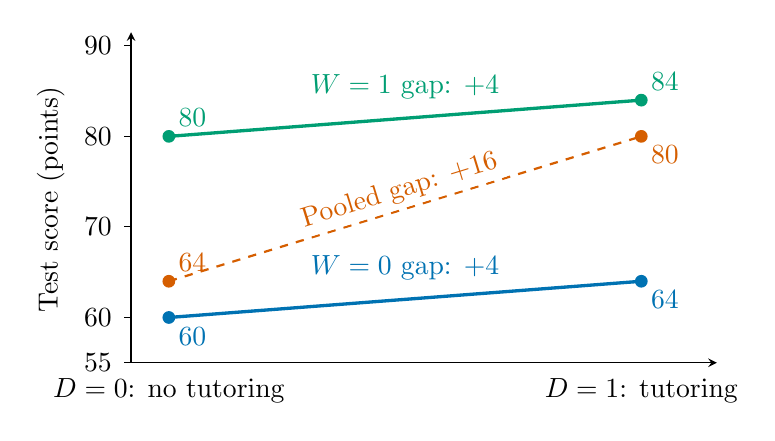
\begin{tikzpicture}[x=6cm,y=.115cm,>=stealth]
\draw[->] (-.08,0)--(1.16,0);
\draw[->] (-.08,0)--(-.08,36.5);
\foreach \y/\lab in {0/55,5/60,15/70,25/80,35/90} {
  \draw (-.08,\y)--(-.095,\y);
  \node[left] at (-.10,\y) {$\lab$};
}
\node[rotate=90] at (-.25,18) {Test score (points)};
\node[below] at (0,-.7) {$D=0$: no tutoring};
\node[below] at (1,-.7) {$D=1$: tutoring};
\draw[blue,very thick] (0,5)--(1,9);
\draw[green,very thick] (0,25)--(1,29);
\draw[red,thick,dashed] (0,9)--(1,25)
  node[midway,above,sloped,fill=white,inner sep=2pt] {Pooled gap: $+16$};
\foreach \x/\y in {0/5,1/9} {\fill[blue] (\x,\y) circle[radius=2.3pt];}
\foreach \x/\y in {0/25,1/29} {\fill[green] (\x,\y) circle[radius=2.3pt];}
\foreach \x/\y in {0/9,1/25} {\fill[red] (\x,\y) circle[radius=2.3pt];}
\node[blue,below right] at (0,5) {$60$};
\node[blue,below right] at (1,9) {$64$};
\node[green,above right] at (0,25) {$80$};
\node[green,above right] at (1,29) {$84$};
\node[red,above right] at (0,9) {$64$};
\node[red,below right] at (1,25) {$80$};
\node[blue,fill=white,inner sep=1pt] at (.5,10.5) {$W=0$ gap: $+4$};
\node[green,fill=white,inner sep=1pt] at (.5,30.5) {$W=1$ gap: $+4$};
\end{tikzpicture}
\end{center}
The pooled line uses each tutoring group's own background mix. Each background-specific line compares students with the same $W$.
\end{frame}
% SOLUTION 2 END
\fi

\begin{frame}{Problem 3: What does holding other regressors fixed mean?}
An estimated school-score equation is
\[
\widehat y=500-1.2M+4E+.5I,
\]
where $M$ is the meal-subsidy share in percentage points, $E$ is average adult schooling in years, and $I$ is annual household income in thousands of euros. Scores are measured in points.
\begin{enumerate}
\setlength{\itemsep}{9pt}
\item Predict scores for school A, $(M,E,I)=(40,12,30)$, and school B, $(50,12,30)$. Which regressors are held fixed?
\item Predict the score for school C, $(50,14,34)$. Decompose the predicted change from A to C into the contributions of $M$, $E$, and $I$. Compare it with the A-to-B change.
\item State the units and ceteris paribus interpretation of each slope. How many slope coefficients and how many total coefficients are estimated?
\end{enumerate}
\end{frame}
\note{All school summaries and coefficients are hypothetical teaching data, not estimates from the California dataset. Solution to Problem 3. Substitute the covariates into the fitted equation: schoolA500-48+48+15=515;schoolB500-60+48+15=503. E and I are held fixed, so A toB isolates a10-percentage-point increase in M and a fitted difference-12. SchoolC500-60+56+17=513. A toC difference is betaM DeltaM+betaE DeltaE+betaI DeltaI=-1.2(10)+4(2)+.5(4)=-12+8+2=-2. The meal coefficient is-1.2 score points per percentage point holding E,I fixed; education coefficient4 points per year holding M,I fixed; income coefficient.5 points per1000 euros holding M,E fixed. There are k3 slopes and4 total coefficients including the500-point intercept. Interpretations describe fitted associations; they do not establish causal effects.}

\ifshowsolutions
% SOLUTION 3 START
\begin{frame}{Solution 3: Partial comparisons and simultaneous changes}
\small
\answerpart{1}Substitute into $\widehat y=\widehat\beta_0+\widehat\beta_MM+\widehat\beta_EE+\widehat\beta_II$:
\begin{align*}
\widehat y_A&=500-1.2(40)+4(12)+.5(30)=\boxed{515},\\
\widehat y_B&=500-1.2(50)+4(12)+.5(30)=\boxed{503}.
\end{align*}
Adult schooling and income are held fixed; $\widehat y_B-\widehat y_A=-12$ points.
\par\vspace{4pt}
\answerpart{2}For school C, $\widehat y_C=500-1.2(50)+4(14)+.5(34)=\boxed{513}$. The change is
\begin{align*}
\Delta\widehat y&=\widehat\beta_M\Delta M+\widehat\beta_E\Delta E+\widehat\beta_I\Delta I\\
&=-1.2(10)+4(2)+.5(4)=-12+8+2=\boxed{-2\text{ points}}.
\end{align*}
\answerpart{3}Each slope describes a fitted association holding the other two regressors fixed:
\begin{center}
\begin{tabular}{c|l}
Slope & Units and interpretation \\ \hline
$-1.2$ on $M$ & $-1.2$ score points per percentage point of meal share \\
$4$ on $E$ & $+4$ score points per additional year of adult schooling \\
$.5$ on $I$ & $+.5$ score points per additional 1,000 euros of income
\end{tabular}
\end{center}
The intercept is 500 points. There are $k=3$ slopes and $k+1=4$ coefficients in total. These fitted associations alone do not establish causality.
\end{frame}
% SOLUTION 3 END
\fi

\section{OLS}

\begin{frame}{Problem 4: Which conditions must a fitted plane satisfy?}
Six observations on two regressors and an outcome are
\begin{center}
\begin{tabular}{c|rrrrrr}
Observation $i$ & 1 & 2 & 3 & 4 & 5 & 6 \\ \hline
$x_i$ & 0 & 0 & 1 & 1 & 2 & 2 \\
$w_i$ & 0 & 1 & 0 & 1 & 0 & 1 \\
$y_i$ & 11 & 12 & 10 & 17 & 15 & 16
\end{tabular}
\end{center}
Fit a plane $\widehat y_i=\widehat\beta_0+\widehat\beta_1x_i+\widehat\beta_2w_i$.
\begin{enumerate}
\setlength{\itemsep}{7pt}
\item Define the squared-error objective $Q(b_0,b_1,b_2)$. Use the chain rule to derive its three first-order conditions, showing the derivative of a residual with respect to each coefficient.
\item For the candidate $(b_0,b_1,b_2)=(10,2,3)$, calculate fitted values and residuals. Verify $\sum_i\widehat u_i=0$, $\sum_ix_i\widehat u_i=0$, and $\sum_iw_i\widehat u_i=0$.
\item Derive the intercept relation from the first condition. Verify it using the sample means and the candidate slopes.
\end{enumerate}
\end{frame}
\note{All observations are hypothetical teaching data. Solution to Problem 4. Residual r_i(b)=yi-b0-b1xi-b2wi and Q=sum r_i squared. Residual derivatives are-1,-xi,-wi; applying the chain rule gives gradient components-2sum r_i,-2sum xi r_i,-2sum wi r_i. At coefficients10,2,3, fitted values are10,13,12,15,14,17;residuals1,-1,-2,2,1,-1. Their sum is0, x-weighted sum0+0-2+2+2-2=0,and w-weighted sum0-1+0+2+0-1=0. Means are xbar1,wbar.5,ybar13.5. Dividing the intercept normal equation by n gives b0hat=ybar-b1hat xbar-b2hat wbar=13.5-2(1)-3(.5)=10. These sample identities alone do not support a causal interpretation.}

\ifshowsolutions
% SOLUTION 4 START
\begin{frame}{Solution 4: Chain-rule derivatives and three normal equations}
\small
\answerpart{1}For a candidate coefficient vector $\mathbf b=(b_0,b_1,b_2)'$, define
\[
r_i(\mathbf b)=y_i-b_0-b_1x_i-b_2w_i,
\qquad Q(\mathbf b)=\sum_{i=1}^n r_i(\mathbf b)^2.
\]
The residual derivatives are
\[
\frac{\partial r_i}{\partial b_0}=-1,
\qquad \frac{\partial r_i}{\partial b_1}=-x_i,
\qquad \frac{\partial r_i}{\partial b_2}=-w_i.
\]
Apply the chain rule, $\partial Q/\partial b_j=\sum_i2r_i(\mathbf b)\,\partial r_i/\partial b_j$, and set the derivatives to zero at the minimum:
\begin{align*}
\frac{\partial Q}{\partial b_0}&=-2\sum_i(y_i-b_0-b_1x_i-b_2w_i)=0,\\[4pt]
\frac{\partial Q}{\partial b_1}&=-2\sum_ix_i(y_i-b_0-b_1x_i-b_2w_i)=0,\\[4pt]
\frac{\partial Q}{\partial b_2}&=-2\sum_iw_i(y_i-b_0-b_1x_i-b_2w_i)=0.
\end{align*}
At OLS, evaluate these equations at $\mathbf b=\widehat{\boldsymbol\beta}$.
\end{frame}

\begin{frame}{Solution 4: Check residuals and recover the intercept (continued)}
\small
\answerpart{2}Use $\widehat y_i=10+2x_i+3w_i$ and $\widehat u_i=y_i-\widehat y_i$:
\begin{columns}[c]
\begin{column}{.51\textwidth}
\begin{center}
\begin{tabular}{c|rrrrr}
$i$ & $x_i$ & $w_i$ & $y_i$ & $\widehat y_i$ & $\widehat u_i$ \\ \hline
1 & 0 & 0 & 11 & 10 & 1 \\
2 & 0 & 1 & 12 & 13 & $-1$ \\
3 & 1 & 0 & 10 & 12 & $-2$ \\
4 & 1 & 1 & 17 & 15 & 2 \\
5 & 2 & 0 & 15 & 14 & 1 \\
6 & 2 & 1 & 16 & 17 & $-1$
\end{tabular}
\end{center}
\end{column}
\begin{column}{.46\textwidth}
\begin{align*}
\sum_i\widehat u_i&=1-1-2+2+1-1=0,\\
\sum_ix_i\widehat u_i&=0+0-2+2+2-2=0,\\
\sum_iw_i\widehat u_i&=0-1+0+2+0-1=0.
\end{align*}
\end{column}
\end{columns}
\answerpart{3}The means are $\overline x=6/6=1$, $\overline w=3/6=.5$, and $\overline y=81/6=13.5$. Divide the intercept condition by $n$:
\[
\sum_i\widehat u_i=0
\quad\Longrightarrow\quad
\overline y-\widehat\beta_0-\widehat\beta_1\overline x-\widehat\beta_2\overline w=0.
\]
\[
\widehat\beta_0=\overline y-\widehat\beta_1\overline x-\widehat\beta_2\overline w
=13.5-2(1)-3(.5)=\boxed{10}.
\]
The normal equations are fitting identities; they do not establish causality.
\end{frame}
% SOLUTION 4 END
\fi

\begin{frame}{Problem 5: How do the scalar conditions become matrices?}
Use the six observations in Problem 4 and the coefficient order $(b_0,b_1,b_2)$ for the intercept, $x$, and $w$.
\begin{enumerate}
\setlength{\itemsep}{11pt}
\item Form the design matrix $\mathbf X$, outcome vector $\mathbf Y$, and coefficient vector $\mathbf b$. Include the intercept column and state all dimensions. What are the dimensions of $\mathbf X\mathbf b$ and $\mathbf Y-\mathbf X\mathbf b$?
\item Compute $\mathbf X'\mathbf X$ and $\mathbf X'\mathbf Y$, showing which sample sums form their entries. State their dimensions.
\item Write the three scalar normal equations represented by $(\mathbf X'\mathbf X)\mathbf b=\mathbf X'\mathbf Y$. Match each row to a first-order condition from Problem 4. Write the gradient of $Q$ in matrix form and check its dimensions.
\end{enumerate}
\end{frame}
\note{All observations are hypothetical teaching data reused explicitly from Problem 4. Solution to Problem 5. X is6 by3 with rows(1,0,0),(1,0,1),(1,1,0),(1,1,1),(1,2,0),(1,2,1). Y is the6 by1 vector(11,12,10,17,15,16) and b is3 by1. Fitted values Xb and residuals Y-Xb are6 by1. XprimeX is3 by3 with rows(6,6,3),(6,10,3),(3,3,3);XprimeY is3 by1 with entries81,89,45. The normal equations are6b0+6b1+3b2=81;6b0+10b1+3b2=89;3b0+3b1+3b2=45. They correspond to the intercept, x, and w conditions. The gradient is-2Xprime(Y-Xb), a3 by1 vector from a3 by6 times6 by1 product. No matrix inverse or coefficient uncertainty calculation is required in this problem.}

\ifshowsolutions
% SOLUTION 5 START
\begin{frame}{Solution 5: Stack observations and keep the intercept column}
\small
\answerpart{1}Each row of the design matrix is $(1,x_i,w_i)$:
\[
\mathbf X_{6\times3}=
\begin{bmatrix}
1&0&0\\
1&0&1\\
1&1&0\\
1&1&1\\
1&2&0\\
1&2&1
\end{bmatrix},
\qquad
\mathbf Y_{6\times1}=
\begin{bmatrix}11\\12\\10\\17\\15\\16\end{bmatrix},
\qquad
\mathbf b_{3\times1}=
\begin{bmatrix}b_0\\b_1\\b_2\end{bmatrix}.
\]
The first column of ones makes every row's fitted value include the intercept:
\[
(\mathbf X\mathbf b)_i=1b_0+x_ib_1+w_ib_2.
\]
Check the matrix multiplication and subtraction:
\[
\underbrace{\mathbf X}_{6\times3}
\underbrace{\mathbf b}_{3\times1}
=\underbrace{\mathbf X\mathbf b}_{6\times1},
\qquad
\underbrace{\mathbf Y-\mathbf X\mathbf b}_{6\times1}
=\begin{bmatrix}r_1(\mathbf b)\\\vdots\\r_6(\mathbf b)\end{bmatrix}.
\]
\end{frame}

\begin{frame}{Solution 5: Cross-products of the data (continued)}
\small
\answerpart{2}Compute the cross-product matrices from the sample sums:
\[
\mathbf X'\mathbf X
=\begin{bmatrix}
n&\sum_ix_i&\sum_iw_i\\
\sum_ix_i&\sum_ix_i^2&\sum_ix_iw_i\\
\sum_iw_i&\sum_ix_iw_i&\sum_iw_i^2
\end{bmatrix}
=\underbrace{\begin{bmatrix}6&6&3\\6&10&3\\3&3&3\end{bmatrix}}_{3\times3},
\]
\[
\mathbf X'\mathbf Y
=\begin{bmatrix}\sum_iy_i\\\sum_ix_iy_i\\\sum_iw_iy_i\end{bmatrix}
=\underbrace{\begin{bmatrix}81\\89\\45\end{bmatrix}}_{3\times1}.
\]
\end{frame}

\begin{frame}{Solution 5: Normal equations and gradient (continued)}
\small
\answerpart{3}The matrix equation $(\mathbf X'\mathbf X)\mathbf b=\mathbf X'\mathbf Y$ contains
\[
\begin{aligned}
6b_0+6b_1+3b_2&=81 &&\quad\text{(intercept: }\sum_i r_i=0\text{)},\\
6b_0+10b_1+3b_2&=89 &&\quad\text{($x$: }\sum_i x_ir_i=0\text{)},\\
3b_0+3b_1+3b_2&=45 &&\quad\text{($w$: }\sum_i w_ir_i=0\text{)}.
\end{aligned}
\]
For $Q(\mathbf b)=(\mathbf Y-\mathbf X\mathbf b)'(\mathbf Y-\mathbf X\mathbf b)$,
\[
\nabla_{\mathbf b}Q=-2\underbrace{\mathbf X'}_{3\times6}
\underbrace{(\mathbf Y-\mathbf X\mathbf b)}_{6\times1}
\quad\text{is }3\times1.
\]
Setting this gradient to zero recovers all three scalar conditions.
\end{frame}
% SOLUTION 5 END
\fi

\begin{frame}{Problem 6: How do we solve the multiple-regression equations?}
Use the design matrix and scores from Problems 4--5, with columns ordered as the intercept, $X$, and $W$:
\[
G=\mathbf X'\mathbf X=\begin{pmatrix}6&6&3\\6&10&3\\3&3&3\end{pmatrix},
\qquad
h=\mathbf X'\mathbf Y=\begin{pmatrix}81\\89\\45\end{pmatrix}.
\]
A proposed inverse is
\[
A=\begin{pmatrix}7/12&-1/4&-1/3\\-1/4&1/4&0\\-1/3&0&2/3\end{pmatrix}.
\]
\begin{enumerate}
\setlength{\itemsep}{7pt}
\item Verify that $GA=I_3$. What does invertibility tell us about the design matrix?
\item Solve the normal equations $G\widehat{\boldsymbol\beta}=h$ by multiplying $Ah$, showing each coefficient calculation.
\item Predict scores at $x=1.5$ for $w=0$ and $w=1$. Interpret the coefficient on $W$ while holding $X$ fixed.
\end{enumerate}
\end{frame}
\note{All numerical quantities are hypothetical teaching data. Solution to Problem 6. Multiplication gives GA=I3. The rows are: first column (7/2-3/2-1,7/2-5/2-1,7/4-3/4-1)=(1,0,0); second column (-3/2+3/2,-3/2+5/2,-3/4+3/4)=(0,1,0); third column (-2+2,-2+2,-1+2)=(0,0,1). Thus A is the inverse of G and the three design columns are linearly independent. The coefficient vector is Ah. Intercept=7(81)/12-89/4-45/3=47.25-22.25-15=10. X slope=-81/4+89/4=2. W slope=-81/3+2(45)/3=3. Fitted scores at x1.5 are 10+2(1.5)+3(0)=13 and 10+2(1.5)+3(1)=16. Holding X fixed, W1 versus W0 has a predicted score difference of 3 points. This is a fitted association and does not by itself establish a causal effect. The inverse is used only to solve the estimation equations.}

\ifshowsolutions
% SOLUTION 6 START
\begin{frame}{Solution 6: Checking the inverse and full column rank}
\small
\answerpart{1}Multiply the proposed inverse by $G$ on the left:
\[
\begin{aligned}
GA&=
\begin{pmatrix}
\frac72-\frac32-1 & -\frac32+\frac32 & -2+2\\[3pt]
\frac72-\frac52-1 & -\frac32+\frac52 & -2+2\\[3pt]
\frac74-\frac34-1 & -\frac34+\frac34 & -1+2
\end{pmatrix}\\[5pt]
&=\begin{pmatrix}1&0&0\\0&1&0\\0&0&1\end{pmatrix}=I_3.
\end{aligned}
\]
Therefore $A=G^{-1}$. Since $G=\mathbf X'\mathbf X$ is invertible, the three columns of $\mathbf X$ are linearly independent: the design has full column rank.

\par\vspace{8pt}
The normal equations consequently have the unique solution
\[
G\widehat{\boldsymbol\beta}=h
\quad\Longrightarrow\quad
\widehat{\boldsymbol\beta}=G^{-1}h=Ah.
\]
\end{frame}

\begin{frame}{Solution 6: The coefficients and controlled predictions}
\small
\answerpart{2}For $j=0,1,2$, $\widehat\beta_j=\sum_{\ell=1}^3 A_{j+1,\ell}h_\ell$. Thus
\[
\begin{aligned}
\widehat\beta_0&=\frac7{12}(81)-\frac14(89)-\frac13(45)
=47.25-22.25-15=\boxed{10},\\[3pt]
\widehat\beta_1&=-\frac14(81)+\frac14(89)+0(45)=\boxed{2},\\[3pt]
\widehat\beta_2&=-\frac13(81)+0(89)+\frac23(45)=\boxed{3}.
\end{aligned}
\]
\answerpart{3}Use $\widehat y(x,w)=\widehat\beta_0+\widehat\beta_1x+\widehat\beta_2w$:
\[
\widehat y(1.5,0)=10+2(1.5)+3(0)=13,
\]
\[
\widehat y(1.5,1)=10+2(1.5)+3(1)=16.
\]
Holding $X$ fixed, changing $W$ from 0 to 1 is associated with a fitted score increase of 3 points. This fitted comparison does not establish causality by itself.
\end{frame}
% SOLUTION 6 END
\fi

\section{Fit}

\begin{frame}{Problem 7: How well does the fitted plane describe scores?}
Return to the six observations in Problems 4--6. The model has an intercept and two regressors, and
\[
n=6,\qquad SSR=12,\qquad TSS_Y=41.5.
\]
\begin{enumerate}
\setlength{\itemsep}{11pt}
\item Count the estimated coefficients and residual degrees of freedom. Compute $SER$ and the in-sample $RMSE$.
\item Find the explained sum of squares, $ESS$, and calculate $R^2$.
\item Calculate adjusted $R^2$ using both the ratio of corrected sums of squares and the expression involving $1-R^2$.
\item Explain why adjusted $R^2$ is no larger than $R^2$ here. State the units of $SER$ and $R^2$ and explain what each measures.
\end{enumerate}
\end{frame}
\note{All numerical quantities are hypothetical teaching data. Solution to Problem 7. k2 excludes the intercept, so there are k+1=3 estimated coefficients and n-k-1=3 residual degrees of freedom. SER=sqrt(SSR/(n-k-1))=sqrt(12/3)=2 score points. In-sample RMSE=sqrt(SSR/n)=sqrt(12/6)=sqrt2=1.41421 points. ESS=TSS-SSR=29.5. R squared=1-12/41.5=59/83=.710843. Adjusted R squared=1-(12/3)/(41.5/5)=1-40/83=43/83=.518072. Equivalently 1-[(n-1)/(n-k-1)](1-R squared)=1-(5/3)(24/83)=43/83. Because (n-1)/(n-k-1)=5/3 exceeds one and 1-R squared is positive, the adjusted statistic is lower. SER describes residual size in score points after a degrees-of-freedom correction; R squared is unitless and describes the share of observed score variation accounted for by the fitted plane. These are sample fit measures and do not by themselves provide a formal prediction interval or causal interpretation.}

\ifshowsolutions
% SOLUTION 7 START
\begin{frame}{Solution 7: Residual size and the unadjusted fit}
\small
\answerpart{1}Here $k=2$ counts regressors other than the intercept:
\[
\text{coefficient count}=k+1=3,
\qquad \text{residual degrees of freedom}=n-k-1=6-2-1=3.
\]
The two residual-size summaries are
\[
SER=\sqrt{\frac{SSR}{n-k-1}}=\sqrt{\frac{12}{3}}=\sqrt4=\boxed{2\text{ points}},
\]
\[
RMSE=\sqrt{\frac{SSR}{n}}=\sqrt{\frac{12}{6}}=\sqrt2\approx1.4142\text{ points}.
\]
\answerpart{2}With an intercept, the sums-of-squares decomposition gives
\[
ESS=TSS_Y-SSR=41.5-12=29.5,
\]
\[
R^2=1-\frac{SSR}{TSS_Y}=1-\frac{12}{41.5}
=\frac{29.5}{41.5}=\boxed{\frac{59}{83}\approx.7108}.
\]
\end{frame}

\begin{frame}{Solution 7: Adjusted fit and units (continued)}
\small
\answerpart{3}First compare the corrected sums of squares:
\[
\overline R^2=1-\frac{SSR/(n-k-1)}{TSS_Y/(n-1)}
=1-\frac{12/3}{41.5/5}
=1-\frac4{8.3}=\boxed{\frac{43}{83}\approx.5181}.
\]
The equivalent formula gives the same value:
\[
\overline R^2
=1-\frac{n-1}{n-k-1}(1-R^2)
=1-\frac53\left(1-\frac{59}{83}\right)
=1-\frac{40}{83}=\frac{43}{83}.
\]
\answerpart{4}The correction multiplies the unexplained share $1-R^2$ by $5/3>1$, so $\overline R^2<R^2$ here.

\par\vspace{8pt}
$SER=2$ is measured in score points and summarizes residual size with a degrees-of-freedom correction. $R^2$ is unitless: the fitted plane accounts for about 71.1\% of the observed variation around the sample mean.

\par\vspace{6pt}
These fit measures alone do not provide a formal prediction interval or establish a causal effect.
\end{frame}
% SOLUTION 7 END
\fi

\begin{frame}{Problem 8: Does adding a control improve the adjusted fit?}
Three OLS models use the same 40 observations and outcome, with $TSS_Y=200$. Each model includes an intercept and has full column rank.
\begin{center}
\begin{tabular}{cclc}
\toprule
Model & Regressor count $k$ & Comparison with A & $SSR$ \\
\midrule
A & 1 & Initial specification & 100 \\
B & 2 & Adds one control & 98 \\
C & 2 & Adds a different control & 90 \\
\bottomrule
\end{tabular}
\end{center}
B and C each nest A; B and C do not nest each other.
\begin{enumerate}
\setlength{\itemsep}{9pt}
\item Calculate $R^2$ and adjusted $R^2$ for all three models.
\item Derive how small the new $SSR$ must be for a one-control expansion of A to improve adjusted $R^2$.
\item Explain why adding a control weakly raises raw $R^2$ but can lower adjusted $R^2$. Can these statistics alone determine the controls needed for a causal analysis?
\end{enumerate}
\end{frame}
\note{All model summaries are hypothetical teaching examples. Solution to Problem 8. With n40, raw R squared=1-SSR/200 and adjusted R squared=1-[SSR/(40-k-1)]/(200/39). A has residual df38, R squared .5, adjusted37/76=.4868421. B has df37, R squared .51, adjusted1789/3700=.4835135. C has df37, R squared .55, adjusted389/740=.5256757. A one-control expansion improves adjusted fit if SSRnew/37<100/38, hence SSRnew<100(37/38)=97.368421. B's SSR98 misses this threshold and adjusted fit falls; C's SSR90 meets it. On the same observations with an intercept, the old fitted model remains feasible after an additional regressor by setting the new coefficient to zero. Minimization therefore cannot raise SSR and cannot lower raw R squared. Adjusted fit also penalizes the lost degree of freedom and may fall. The comparison establishes fit consequences, not which controls identify a causal effect. B and C have different extra controls and are not nested with one another.}

\ifshowsolutions
% SOLUTION 8 START
\begin{frame}{Solution 8: Comparing raw and adjusted fit}
\small
\answerpart{1}For each model,
\[
R^2=1-\frac{SSR}{TSS_Y},
\qquad
\overline R^2=1-\frac{SSR/(n-k-1)}{TSS_Y/(n-1)}.
\]
With $TSS_Y=200$ and $n=40$:
\begin{center}
\begin{tabular}{c|rrrrr}
Model & $k$ & $SSR$ & $n-k-1$ & $R^2$ & $\overline R^2$ \\
\hline
A & 1 & 100 & 38 & $.5000$ & $.4868$ \\
B & 2 & 98 & 37 & $.5100$ & $.4835$ \\
C & 2 & 90 & 37 & $.5500$ & $.5257$
\end{tabular}
\end{center}
For example, the adjusted calculations are
\[
\begin{aligned}
\overline R_A^2&=1-\frac{100/38}{200/39}=\frac{37}{76}\approx.4868,\\
\overline R_B^2&=1-\frac{98/37}{200/39}=\frac{1789}{3700}\approx.4835,\\
\overline R_C^2&=1-\frac{90/37}{200/39}=\frac{389}{740}\approx.5257.
\end{aligned}
\]
\end{frame}

\begin{frame}{Solution 8: The improvement threshold and control selection}
\small
\answerpart{2}The denominator $TSS_Y/(n-1)$ is common to the models. Therefore,
\[
\begin{aligned}
\overline R_{\mathrm{new}}^2>\overline R_A^2
&\iff \frac{SSR_{\mathrm{new}}}{40-2-1}<\frac{100}{40-1-1}\\
&\iff SSR_{\mathrm{new}}<100\frac{37}{38}
\approx\boxed{97.3684}.
\end{aligned}
\]
B's $SSR=98$ fails this threshold; C's $SSR=90$ satisfies it.
\par\vspace{8pt}
\answerpart{3}In an expanded model, setting the new coefficient to zero reproduces the old fitted values. On the same observations, minimized $SSR$ can only fall or stay unchanged, so raw $R^2$ can only rise or stay unchanged.

\par\vspace{6pt}
Adjusted $R^2$ also accounts for the lost degree of freedom. A small reduction in $SSR$ may not compensate for this penalty, as model B shows.

\par\vspace{6pt}
Causal controls must be chosen using the identification argument and knowledge of the variables. Fit statistics alone cannot determine the appropriate causal specification.
\end{frame}
% SOLUTION 8 END
\fi

\begin{frame}{Problem 9: How can adjusted R-squared be negative?}
An OLS regression uses $n=10$ observations, an intercept, and $k=3$ regressors. The design has full column rank, and
\[
TSS_Y=90,\qquad SSR=80.
\]
Scores are measured in points.
\begin{enumerate}
\setlength{\itemsep}{13pt}
\item Calculate raw $R^2$ and adjusted $R^2$.
\item Calculate $RMSE$, $SER$, and the sample variance $s_Y^2$. Which comparison explains the sign of adjusted $R^2$?
\item An intercept-only regression on the same observations has $SSR=90$. Calculate its adjusted $R^2$ and compare its corrected residual average with that of the larger model. Why can a model with lower $SSR$ have worse adjusted fit?
\end{enumerate}
\end{frame}
\note{All model summaries are hypothetical teaching examples. Solution to Problem 9. The full model has 10-3-1=6 residual degrees of freedom. Raw R squared=1-80/90=1/9=.111111. Adjusted R squared=1-(80/6)/(90/9)=1-4/3=-1/3. In-sample RMSE=sqrt(80/10)=sqrt8=2.828427 score points. SER=sqrt(80/6)=sqrt(40/3)=3.651484 points. Sample outcome variance=90/(10-1)=10 points squared; SER squared=40/3 exceeds10. The negative adjusted statistic reflects this corrected residual average exceeding the outcome's corrected sum of squares per degree of freedom. It does not mean raw explained variation is negative. For the intercept-only model k0, residual df9, SSR90, raw R squared0 and adjusted R squared=1-(90/9)/(90/9)=0. The three additional regressors reduce SSR from90 to80, but reduce residual degrees of freedom from9 to6. Thus corrected residual average rises from10 to13.3333, so adjusted fit is lower. This comparison does not by itself select the controls needed for causal identification.}

\ifshowsolutions
% SOLUTION 9 START
\begin{frame}{Solution 9: Raw fit, adjusted fit, and residual size}
\small
\answerpart{1}With $n-k-1=10-3-1=6$,
\[
R^2=1-\frac{SSR}{TSS_Y}=1-\frac{80}{90}=\boxed{\frac19\approx.1111},
\]
\[
\overline R^2=1-\frac{SSR/(n-k-1)}{TSS_Y/(n-1)}
=1-\frac{80/6}{90/9}=1-\frac43=\boxed{-\frac13}.
\]
\answerpart{2}The residual-size summaries and outcome variance are
\[
RMSE=\sqrt{\frac{SSR}{n}}=\sqrt{\frac{80}{10}}=\sqrt8\approx2.8284\text{ points},
\]
\[
SER=\sqrt{\frac{SSR}{n-k-1}}=\sqrt{\frac{80}{6}}\approx3.6515\text{ points},
\qquad
s_Y^2=\frac{TSS_Y}{n-1}=\frac{90}{9}=10\text{ points}^2.
\]
Because $SER^2=80/6>10=s_Y^2$, their ratio exceeds one and adjusted $R^2$ is negative. Raw explained variation remains nonnegative.
\end{frame}

\begin{frame}{Solution 9: The intercept-only benchmark (continued)}
\small
\answerpart{3}The intercept-only model estimates one coefficient, the sample mean. With $k=0$, its residual degrees of freedom are $n-1=9$:
\[
\overline R_{\mathrm{intercept}}^2
=1-\frac{SSR/(n-1)}{TSS_Y/(n-1)}
=1-\frac{90/9}{90/9}=\boxed{0}.
\]
Compare the corrected residual averages:
\[
\frac{SSR_{\mathrm{intercept}}}{9}=\frac{90}{9}=10,
\qquad
\frac{SSR_{\mathrm{larger}}}{6}=\frac{80}{6}=13\tfrac13.
\]
The larger model reduces $SSR$ by 10, but uses three additional coefficients. Its reduction in squared residuals is too small to offset the loss of residual degrees of freedom.

\par\vspace{8pt}
A negative adjusted $R^2$ is possible because it is a penalized fit statistic. This comparison alone does not determine the controls needed for a causal analysis.
\end{frame}
% SOLUTION 9 END
\fi

\section{Inference}

\begin{frame}{Problem 10: What do the coefficient variances tell us?}
A regression using a large i.i.d. sample of $n=200$ observations estimates
\[
Y=\beta_0+\beta_1X+\beta_2W+U,
\qquad
\widehat{\boldsymbol\beta}=\begin{pmatrix}2\\1.5\\-.8\end{pmatrix}.
\]
An appropriate estimated coefficient covariance matrix, ordered as the intercept, $X$, and $W$, is supplied:
\[
\widehat V=\begin{pmatrix}.25&.02&-.01\\.02&.36&.04\\-.01&.04&.16\end{pmatrix}.
\]
Use the large-sample normal approximation, $z_{.975}=1.96$, $\Phi(2.5)=.9938$, and $\Phi(2)=.97725$.
\begin{enumerate}
\setlength{\itemsep}{7pt}
\item Read off the estimated variances and covariances, and calculate all three coefficient standard errors.
\item Test each slope separately against zero using a two-sided 5\% test. Compute both $p$-values.
\item Construct the two 95\% slope confidence intervals. Relate zero's membership to the tests, and state what the results establish.
\end{enumerate}
\end{frame}
\note{All numerical estimates and the supplied appropriate covariance matrix are hypothetical teaching quantities. Solution to Problem 10. The supplied matrix is treated as a valid estimated covariance matrix; students do not derive it. Diagonal entries are the estimated variances of the intercept .25, X slope .36, and W slope .16. Their standard errors are the square roots .5,.6,.4. Off-diagonal estimated covariances are .02 for intercept and X slope, -.01 for intercept and W slope, and .04 for the two slopes. For H0 beta1 zero versus nonzero, t=1.5/.6=2.5, p=2(1-.9938)=.0124. For H0 beta2 zero versus nonzero, t=-.8/.4=-2, p=2(1-.97725)=.0455. Reject both separate nulls at5 percent using the large-sample normal approximation. X slope CI=1.5 plus or minus1.96(.6)=[.324,2.676]; W slope CI=-.8 plus or minus1.96(.4)=[-1.584,-.016]. Neither includes zero, agreeing with the corresponding two-sided test. These are separate slope tests and intervals describing controlled associations, not a joint test and not automatic evidence of a causal effect. No exact small-sample distribution is assumed.}

\ifshowsolutions
% SOLUTION 10 START
\begin{frame}{Solution 10: Reading variances and forming separate tests}
\small
\answerpart{1}For coefficient $j$, $\widehat{\Var}(\widehat\beta_j)=\widehat V_{j+1,j+1}$ and $SE(\widehat\beta_j)=\sqrt{\widehat V_{j+1,j+1}}$. Thus
\[
\begin{array}{c|ccc}
\text{Coefficient} & \widehat\beta_0 & \widehat\beta_1 & \widehat\beta_2\\\hline
\text{Estimated variance} & .25 & .36 & .16\\
\text{Standard error} & \sqrt{.25}=.50 & \sqrt{.36}=.60 & \sqrt{.16}=.40
\end{array}
\]
The estimated covariances are
\[
\widehat{\Cov}(\widehat\beta_0,\widehat\beta_1)=.02,\quad
\widehat{\Cov}(\widehat\beta_0,\widehat\beta_2)=-.01,\quad
\widehat{\Cov}(\widehat\beta_1,\widehat\beta_2)=.04.
\]
\answerpart{2}For each $j=1,2$, test $H_0:\beta_j=0$ against $H_1:\beta_j\ne0$, using
\[
t_j=\frac{\widehat\beta_j-0}{SE(\widehat\beta_j)},
\qquad p_j\approx2[1-\Phi(|t_j|)].
\]
\[
\begin{aligned}
t_1&=\frac{1.5}{.60}=2.5,&p_1&\approx2(1-.9938)=.0124,\\
t_2&=\frac{-.8}{.40}=-2,&p_2&\approx2(1-.97725)=.0455.
\end{aligned}
\]
Both separate nulls are rejected at 5\%: $|t_j|>1.96$ and $p_j<.05$.
\end{frame}

\begin{frame}{Solution 10: Slope confidence intervals and interpretation}
\small
\answerpart{3}For each slope, the large-sample 95\% interval is
\[
\widehat\beta_j\pm1.96\,SE(\widehat\beta_j).
\]
For the coefficient on $X$,
\[
1.5\pm1.96\sqrt{.36}
=1.5\pm1.96(.60)
=1.5\pm1.176=\boxed{[.324,\ 2.676]}.
\]
For the coefficient on $W$,
\[
-.8\pm1.96\sqrt{.16}
=-.8\pm1.96(.40)
=-.8\pm.784=\boxed{[-1.584,\ -.016]}.
\]
Neither interval contains zero, agreeing with rejection in each corresponding two-sided 5\% test.

\par\vspace{8pt}
The estimated association with $X$ is positive holding $W$ fixed; the estimated association with $W$ is negative holding $X$ fixed. These are separate coefficient tests and intervals, not a joint test. A causal interpretation requires an identification argument beyond these results.
\end{frame}
% SOLUTION 10 END
\fi

\section{Controls}

\begin{frame}{Problem 11: Can two measures of study time have separate coefficients?}
Regress $Y$ on an intercept, study hours $X_1$, and study minutes $X_2$:
\begin{center}
\begin{tabular}{c|rrrrr}
$x_{1i}$ & 1 & 2 & 3 & 4 & 5\\
$x_{2i}$ & 60 & 120 & 180 & 240 & 300\\
$y_i$ & 15 & 20 & 25 & 30 & 35
\end{tabular}
\end{center}
\begin{enumerate}
\setlength{\itemsep}{7pt}
\item Show the exact relation among the regressor columns. Why is the design matrix's $\mathbf X'\mathbf X$ not invertible?
\item Which combination of the two slope coefficients is identified? Check that $(b_1,b_2)=(5,0)$, $(2,.05)$, and $(-1,.1)$ give the same fitted values when $b_0=10$. What happens if we drop study minutes?
\item Replace the minutes data by $(60,121,179,241,300)$. Is there still an exact affine relation with hours? Does the new design have full column rank? Distinguish this case from perfect multicollinearity and count the residual degrees of freedom.
\end{enumerate}
\end{frame}
\note{All observations are invented for teaching. Solution to Problem 11. Original x2=60x1. With design X=[1,x1,x2], the nonzero vector v=(0,-60,1)' satisfies Xv=0, so X'Xv=0 and X'X is singular. The regression line equals b0+(b1+60b2)x1. The data identify b0=10 and b1+60b2=5, not b1 and b2 separately. Each listed pair satisfies this restriction and fits every observed score exactly. Drop minutes to recover yhat=10+5x1. In perturbed data, points at hours1 and5 force any proposed affine relation x2=a+bx1 to have a0 and b60; the second point contradicts it because121 is not120. Since hours vary, all three columns are independent. There are5 observations and3 independently estimated coefficients, giving2 residual degrees of freedom. The perturbed regressor correlation is approximately .999961, but not perfect. The exact outcome line is still fitted by10+5x1+0x2 in this sample. In noisy samples, near collinearity can make separate coefficient estimates imprecise and sensitive; high regressor correlation is not by itself a source of bias. No uncertainty formula is needed.}

\ifshowsolutions
% SOLUTION 11 START
\begin{frame}{Solution 11: One dimension of study time, two columns}
\small
\answerpart{1}The columns satisfy $x_{2i}-60x_{1i}=0$ for every observation. For the design matrix $\mathbf X=[\mathbf1,\mathbf x_1,\mathbf x_2]$,
\[
v=\begin{pmatrix}0\\-60\\1\end{pmatrix}\ne0,
\qquad \mathbf Xv=0\quad\Longrightarrow\quad \mathbf X'\mathbf Xv=0.
\]
Thus $\mathbf X'\mathbf X$ has a nonzero null vector and is not invertible.
\par\vspace{6pt}
\answerpart{2}Substitute the column relation into any candidate fitted line:
\[
b_0+b_1x_1+b_2x_2=b_0+(b_1+60b_2)x_1.
\]
The data identify $b_0=10$ and $\boxed{b_1+60b_2=5}$. They do not identify the two slopes separately:
\[
5+60(0)=5,\qquad 2+60(.05)=5,\qquad -1+60(.1)=5.
\]
Each coefficient pair produces $\widehat y=10+5x_1$ and the same zero residuals. Dropping the minutes regressor gives the unique simple-regression fit $\boxed{\widehat y=10+5x_1}$.
\end{frame}

\begin{frame}{Solution 11: Near collinearity permits separate coefficients (continued)}
\small
\answerpart{3}Suppose the new minutes column satisfied $x_2=a+bx_1$. Its first and fifth observations would imply
\[
60=a+b,\qquad 300=a+5b
\quad\Longrightarrow\quad b=60,\ a=0.
\]
But at the second observation this relation predicts $x_2=120$, whereas the new value is 121. Hence no exact affine relation holds.
\par\vspace{8pt}
Hours are nonconstant, and minutes cannot be written as a constant plus hours. The three columns therefore have full column rank. With three coefficients,
\[
\text{residual degrees of freedom}=n-3=5-3=\boxed2.
\]
The columns remain extremely similar, so this is \textbf{near collinearity}, rather than perfect multicollinearity.
\par\vspace{8pt}
High correlation among regressors does not itself create bias. In data with noise, however, it can make the separate coefficient estimates imprecise and sensitive to small changes. In these particular data, $\widehat y=10+5x_1+0x_2$ still fits exactly.
\end{frame}
% SOLUTION 11 END
\fi

\begin{frame}{Problem 12: Which category should be the reference group?}
A sample contains four graduates from each of three university categories. Every graduate belongs to exactly one category. Their mean hourly wages are
\begin{center}
\begin{tabular}{c|rrr}
Category & Public & Private & Other\\ \hline
Mean wage (euros/hour) & 18 & 24 & 20
\end{tabular}
\end{center}
Let $P$, $R$, and $O$ be the corresponding category dummies.
\begin{enumerate}
\setlength{\itemsep}{6pt}
\item Why is a regression on an intercept and all three dummies not identified?
\item Omit the public dummy. Find the intercept and the coefficients on the private and other dummies.
\item Use private universities as the reference category instead. Find all coefficients and check predictions for the three categories.
\item Omit the intercept and retain all three dummies. Find the coefficients. Explain why these valid specifications have the same fitted values. Do the wage gaps automatically measure causal effects?
\end{enumerate}
\end{frame}
\note{All group summaries are invented for teaching. Solution to Problem 12. Mutually exclusive exhaustive dummies satisfy P+R+O=1, so intercept plus all three creates an exact column relation. With all groups observed, each valid dummy specification identifies the same three fitted group means. An OLS group-specific constant equals the group's sample mean. Omitting public: intercept18, private6, other2. Omitting private: intercept24, public-6, other-4; predictions public24-6=18, private24, other24-4=20. No intercept with all three: coefficients18,24,20. Reference changes affect coefficient interpretation but not fitted means, residuals, or any pairwise group gap. These are descriptive group differences; without a credible assignment/design argument they do not establish causal university effects.}

\ifshowsolutions
% SOLUTION 12 START
\begin{frame}{Solution 12: A column relation and a public reference group}
\small
\answerpart{1}For every graduate, exactly one dummy is one:
\[
P_i+R_i+O_i=1.
\]
The intercept column equals the sum of all three dummy columns, creating perfect multicollinearity. Four separate coefficients cannot identify only three group means.
\par\vspace{8pt}
\answerpart{2}For group-specific fitted constants $m_g$, OLS minimizes
\[
\sum_g\sum_{i\in g}(y_i-m_g)^2,
\qquad \frac{\partial Q}{\partial m_g}=-2\sum_{i\in g}(y_i-m_g)=0
\quad\Longrightarrow\quad m_g=\overline y_g.
\]
With public omitted, $\widehat y=b_0+b_RR+b_OO$. Therefore
\[
\boxed{b_0=\overline y_P=18},\qquad
\boxed{b_R=\overline y_R-\overline y_P=24-18=6},
\]
\[
\boxed{b_O=\overline y_O-\overline y_P=20-18=2}.
\]
The intercept is the public-group mean; each dummy coefficient is a gap from that reference group, in euros per hour.
\end{frame}

\begin{frame}{Solution 12: Changing the reference preserves fitted wages (continued)}
\small
\answerpart{3}With private omitted, $\widehat y=c_0+c_PP+c_OO$:
\[
\boxed{c_0=24},\qquad
\boxed{c_P=18-24=-6},\qquad
\boxed{c_O=20-24=-4}.
\]
\begin{center}
\begin{tabular}{c|ccc}
Category & Public & Private & Other\\ \hline
Prediction & $24-6=18$ & $24$ & $24-4=20$
\end{tabular}
\end{center}
\answerpart{4}Without an intercept, write $\widehat y=a_PP+a_RR+a_OO$. Each coefficient directly equals its group's fitted mean:
\[
\boxed{a_P=18},\qquad\boxed{a_R=24},\qquad\boxed{a_O=20}.
\]
All three valid parameterizations reproduce the same group means, so they have the same fitted values and residuals. Changing the reference changes the labels and interpretation of coefficients, rather than the fit.
\par\vspace{8pt}
The wage gaps are descriptive. They do not automatically identify causal effects of attending a particular university category.
\end{frame}
% SOLUTION 12 END
\fi

\begin{frame}{Problem 13: Can a useful control have a noncausal coefficient?}
Consider the structural model
\[
Y=10+4D+2W+U,
\qquad \E(U\mid D,W)=3W,
\]
where $D$ is binary participation and $W$ is a binary background characteristic. All four $(D,W)$ cells have positive probability, and variables have finite second moments. The model stipulates that changing $D$ while holding $W$ and $U$ fixed changes $Y$ by 4.
\begin{enumerate}
\setlength{\itemsep}{7pt}
\item Tabulate $\E(U\mid D,W)$ for the four cells. Does conditional mean independence, $\E(U\mid D,W)=\E(U\mid W)$, hold? Does full zero conditional mean hold?
\item Derive $\E(Y\mid D,W)$ and the within-$W$ participation gap. Explain why the binary control absorbs the background-dependent error mean exactly.
\item Which population regression coefficient targets the stipulated causal participation effect? Why need the control coefficient not equal its structural coefficient of 2?
\end{enumerate}
\end{frame}
\note{All model values are invented for teaching. Solution to Problem 13. The structural model explicitly stipulates the causal D effect4. At W0, both D error means0;atW1,both3. By iterated expectations E(U|W)=3W, so conditional mean independence holds despite E(U|D,W) being nonzero at W1. The CEF equals10+4D+5W. Each within-W D gap is4. Because W is binary, an intercept and W fully absorb any function of W; here that function is3W. Defining V=U-3W gives E(V|D,W)=0 and Y=10+4D+5W+V. Thus the population regression on an intercept,D,W has coefficient4 on D and5 onW; under appropriate sampling a sample OLS coefficient on D targets4. The W coefficient combines the stipulated structural2 with the background-linked unobserved-mean3 and is not automatically a causal W effect. CMI for arbitrary continuous W alone would not make an incorrectly specified linear control sufficient; the binary control here represents the error-mean function exactly.}

\ifshowsolutions
% SOLUTION 13 START
\begin{frame}{Solution 13: Conditional mean independence is sufficient here}
\small
\answerpart{1}The conditional error means do not change with $D$ at a given $W$:
\begin{center}
\begin{tabular}{c|cc}
$\E(U\mid D,W)$ & $D=0$ & $D=1$\\ \hline
$W=0$ & 0 & 0\\
$W=1$ & 3 & 3
\end{tabular}
\end{center}
Iterated expectations gives $\E(U\mid W)=\E[3W\mid W]=3W$. Hence
\[
\boxed{\E(U\mid D,W)=\E(U\mid W)}.
\]
Conditional mean independence holds, but full zero conditional mean fails at $W=1$.
\par\vspace{6pt}
\answerpart{2}Taking conditional expectations of the structural equation,
\begin{align*}
\E(Y\mid D,W)
&=10+4D+2W+\E(U\mid D,W)\\
&=10+4D+2W+3W=\boxed{10+4D+5W}.
\end{align*}
For either $w=0$ or $w=1$, the participation gap is
\[
\E(Y\mid D=1,W=w)-\E(Y\mid D=0,W=w)=\boxed4.
\]
\end{frame}

\begin{frame}{Solution 13: The participation and control coefficients differ (continued)}
\small
\answerpart{2}An intercept and binary $W$ can represent any function of $W$:
\[
g(W)=g(0)+[g(1)-g(0)]W.
\]
Here the omitted-factor mean $g(W)=3W$ is absorbed exactly by the control coefficient. Define $V=U-3W$; then
\[
Y=10+4D+5W+V,\qquad\E(V\mid D,W)=0.
\]
\answerpart{3}The population regression coefficient on $D$ is $\boxed4$, which equals the causal participation effect stipulated by this model. Conditioning on $W$ removes the participation-related difference in the mean of $U$.
\par\vspace{8pt}
The population coefficient on $W$ is instead
\[
\boxed5=\underbrace{2}_{\text{structural coefficient}}
+\underbrace{3}_{\text{background-linked error mean}}.
\]
That control coefficient need not measure the causal effect of changing $W$. A useful control does not make every regression coefficient causal.
\par\vspace{8pt}
The exact absorption above uses binary $W$. With other controls, the functional form must represent the relevant background-dependent mean adequately.
\end{frame}
% SOLUTION 13 END
\fi

\begin{frame}{Problem 14: When does a control fail to remove selection?}
Keep the structural model and the causal participation effect of 4, but change the error mean:
\[
Y=10+4D+2W+U,
\qquad\E(U\mid D,W)=3W+2D.
\]
$D$ and $W$ are binary, all four cells have positive probability, and observations are i.i.d. with bounded variables and a full-rank regression design.
\begin{enumerate}
\setlength{\itemsep}{10pt}
\item Tabulate $\E(U\mid D,W)$. At each value of $W$, does its mean depend on participation? Does conditional mean independence hold?
\item Derive $\E(Y\mid D,W)$. Compare the population multiple-regression coefficient on $D$ with its structural causal effect.
\item Would more observations, finite fourth moments, and full rank repair the discrepancy? Identify the failing condition and explain what further design evidence or pre-treatment controls would be needed for a credible causal interpretation.
\end{enumerate}
\end{frame}
\note{All model values are invented for teaching. Solution to Problem 14. Conditional U table with rowsW0,W1 and columnsD0,D1 is0,2;3,5. At both W values the mean differs by2 between participants and nonparticipants. Therefore E(U|D,W)=E(U|W) fails. Conditional outcome mean is10+4D+2W+3W+2D=10+6D+5W. Its D slope6 differs from the structural causal effect4 by2. Define projection error V=U-3W-2D to see E(V|D,W)=0; this property of the observational regression does not restore causal interpretation of6. With iid finite moments and full rank, larger samples target this observational coefficient rather than4. Bounded variables ensure finite fourth moments but do not establish conditional mean independence. A credible design would need to remove the within-W participation-related omitted-factor mean, for example a defensible as-if-random assignment argument within adequate background groups. Additional relevant pre-treatment controls help only if they make the required conditional independence credible and are represented adequately; simply adding controls, observations, or category variation is not a guarantee.}

\ifshowsolutions
% SOLUTION 14 START
\begin{frame}{Solution 14: Selection remains within each background group}
\small
\answerpart{1}The new conditional error means are
\begin{center}
\begin{tabular}{c|cc|c}
$\E(U\mid D,W)$ & $D=0$ & $D=1$ & Difference $(D=1)-(D=0)$\\ \hline
$W=0$ & 0 & 2 & 2\\
$W=1$ & 3 & 5 & 2
\end{tabular}
\end{center}
The error mean changes with $D$ even after fixing $W$. Conditional mean independence therefore fails.
\par\vspace{7pt}
\answerpart{2}Taking conditional expectations,
\begin{align*}
\E(Y\mid D,W)
&=10+4D+2W+\E(U\mid D,W)\\
&=10+4D+2W+3W+2D=\boxed{10+6D+5W}.
\end{align*}
The population observational coefficient on $D$ is $\boxed6$, while the stipulated structural causal effect is $\boxed4$. The remaining within-$W$ selection adds 2 to the participation gap.
\end{frame}

\begin{frame}{Solution 14: Selection and sample size (continued)}
\small
\answerpart{3}I.i.d. sampling, finite fourth moments, and full rank do not imply
\[
\E(U\mid D,W)=\E(U\mid W).
\]
This conditional mean independence condition fails in the stated model. More observations estimate the observational coefficient of 6 more closely; they do not change it into the structural effect of 4.
\par\vspace{10pt}
For a causal interpretation, we would need credible evidence that participation no longer selects on omitted determinants of $Y$ within the relevant background groups. A defensible assignment mechanism or sufficiently informative pre-treatment controls could support that argument.
\par\vspace{10pt}
Additional controls help only when they address the source of selection and represent the relevant conditional means adequately. The number of controls is not evidence that the selection problem has been removed.
\end{frame}
% SOLUTION 14 END
\fi

\end{document}
